\documentclass{report}
\usepackage{hyperref}
\usepackage[ngerman]{babel}
\usepackage{amsmath}
\usepackage{amsfonts}
\usepackage{amsthm}
\usepackage{tcolorbox}
\usepackage[a4paper, total={7in, 9in}]{geometry}
\usepackage[font={scriptsize,it}]{caption}
\usepackage{scrextend}
\usepackage{graphicx}
\usepackage{caption}
\usepackage{subcaption}
\usepackage[utf8]{inputenc}
\usepackage[T1]{fontenc}
\DeclareUnicodeCharacter{2212}{-}
\usepackage{verbatim}
\usepackage{tikz}

\tikzset{
  treenode/.style = {shape=rectangle, rounded corners,
                     draw, align=center,
                     top color=white, bottom color=blue!20},
  root/.style     = {treenode, font=\Large, bottom color=red!30},
  env/.style      = {treenode, font=\ttfamily\normalsize},
  dummy/.style    = {circle,draw}
}

\tikzstyle{level 1}=[level distance=3.5cm, sibling distance=3.5cm]
\tikzstyle{level 2}=[level distance=3.5cm, sibling distance=2cm]

% floating figure for column
\newenvironment{Figure}
	{\par\medskip\noindent\minipage{\linewidth}}
	{\endminipage\par\medskip}

\begin{document}

\begin{titlepage}
   \vspace*{\stretch{1.0}}
   \begin{center}
      \Large\textbf{eHealth Lab05 - HS20}\\
      \large\textit{Results from Pascal Brunner - brunnpa7}
   \end{center}
   \vspace*{\stretch{2.0}}
\end{titlepage}

% Beispiel Bild
%\begin{Figure}
%   \centering
%    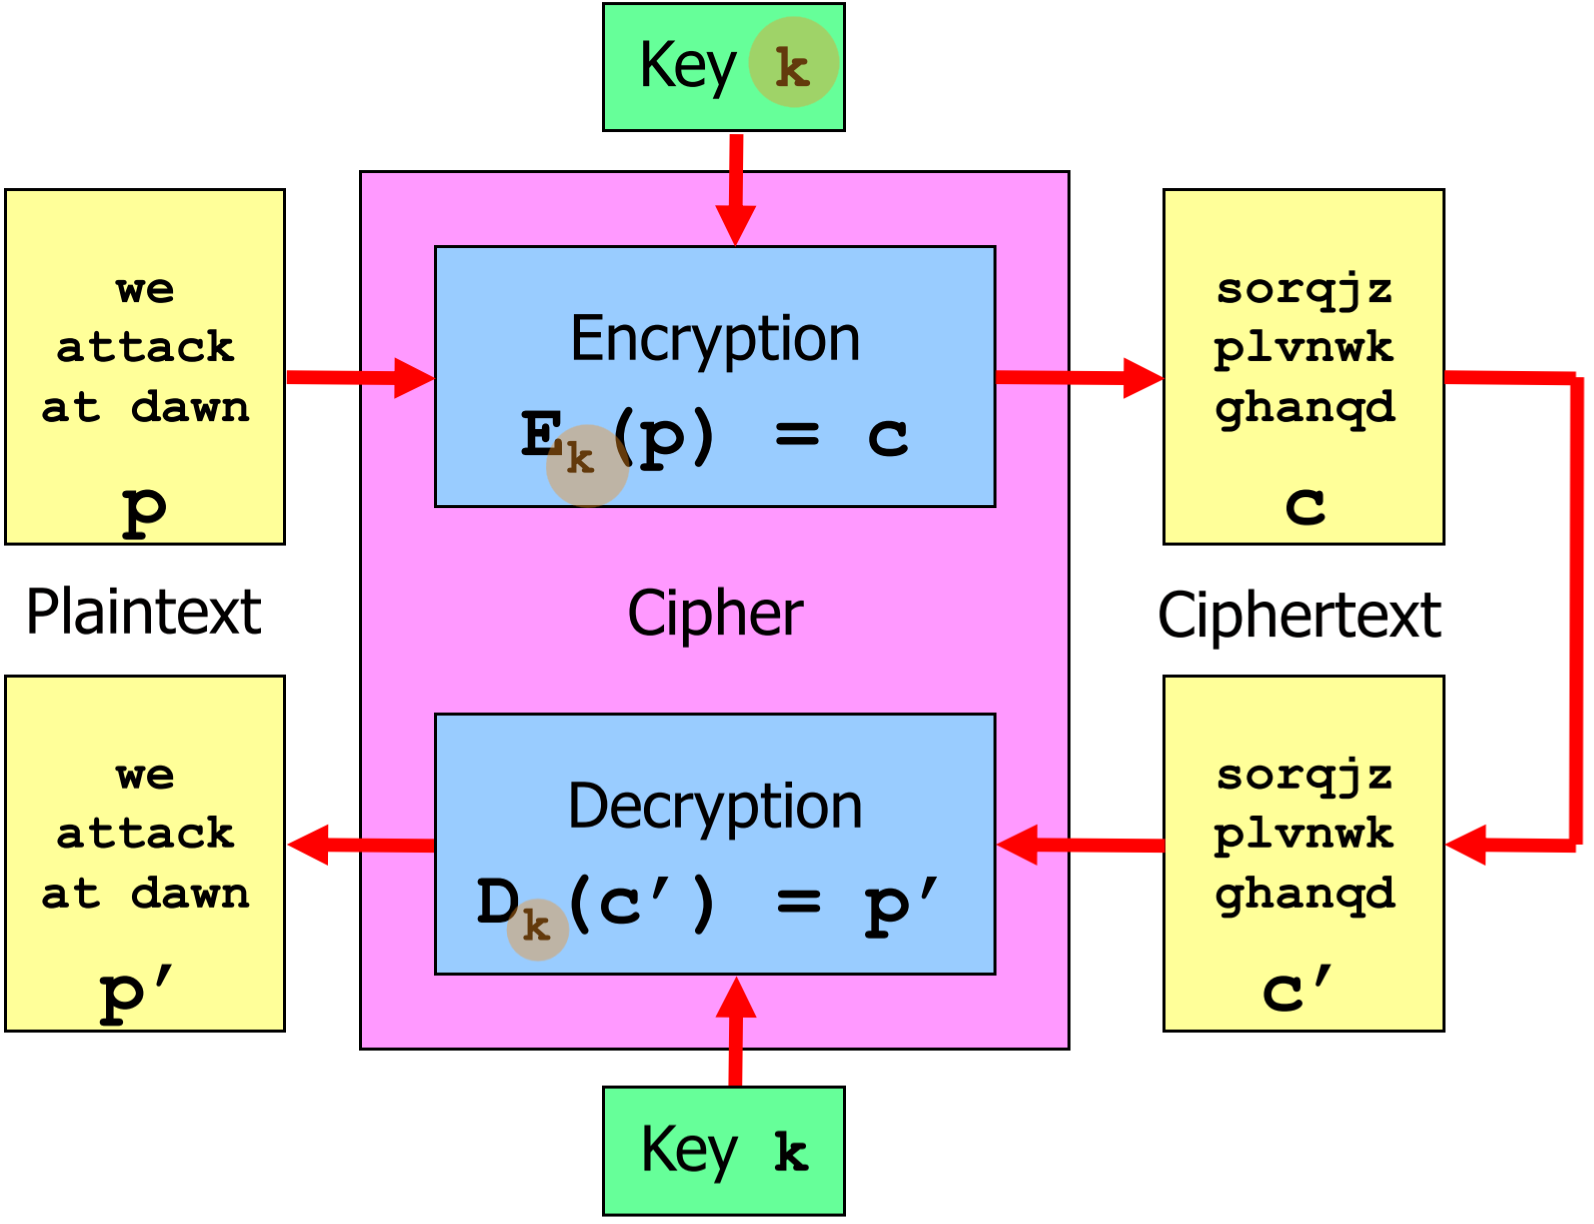
\includegraphics[width=150px]{img/BasicTerminologySecKeyCrypto.png}
%        \captionof{figure}{Basic Terminology basierend auf Secret Key Cryptography}
%        \label{fig:Basic Terminology}
%    \end{Figure}

\section*{Summary what impressed me the most from ICU Cockpit Project at USZ}

While attending the lecture of eHealth, I often thought that surely a lot can be improved by visualizations and the use of artificial intelligence. Especially the recognition of images (e.g. x-ray images) I saw as predestined for this application. \\

Watching the YouTube movie about the ICU cockpit, I was very surprised. On the one hand it is the amount of data that is collected daily per patient. Especially in the intensive care units with an unbelievable number of devices that are connected. 
I thought to myself that as a human being you can hardly keep an overview of all data and all patients. As we heard in the lecture, to err is human - but to err when human life is at stake should of course be kept to a minimum. 
For this reason I find the approach of the ICU Cockpit phenomenal. On the one hand the two presented apps:\\
Smart Alarms:\\ 
I am convinced that if we continue to work on it and improve the 12.8\% false positive rate, we will be able to achieve even better results. Then it is a real game-changer when about 1/3 of alarms can be eliminated - 
because every alarm eats resources and if they are aggregated "wrongly", then these resources can be missing at another place.\\

Stable State:\\
I also find this app impressive. It allows to visualize super complex interactions of various measuring stations in a simple way. We have often heard and learned that visualizations are much easier for humans to interpret than mere numbers and data.\\

Last but not least, I am fascinated by the ICU Cockpit - I am absolutely convinced that such visualizations lead to an improved service in hospitals and therefore more patients are saved and cared for. 
Especially in the current time when hospitals are basically overloaded, the employees can be relieved and thus be focused on the necessary patients


\end{document}